\chapter{Systematic Error Analysis}
\minitoc
\label{Cap:ErrorAnalysis}

The MINER$\nu$A experiment implements the \textit{Many-Universes Uncertainty} method to calculate the error propagation in the cross section process. This method consist of shifting the simulation $\pm\sigma$ for a specific parameter or central value. For each parameter there are two universes one for the $+\sigma$ on other for $-\sigma$ shift. The parameters are shifted based on their associated errors; for example, if the energy of a hadron candidate is estimated by Bethe-Bloch, the reconstructed energy will be shifted by $\pm30$ MeV in this two universes. For the case of the flux uncertainty is repeated 100 times for the reason that it is explained below. These universes produce their own histograms for each variable, which are used to obtain a covariance matrix. For this, an average distribution is calculated by using all the universes, including the central value (CV) universe. The covariance matrix is a square matrix obtained as follow:

\begin{equation}
    C_{ij}=\frac{1}{N}\sum^N_n((u_{i,n}-\Bar{u}_{i})-(u_{j,n}-\Bar{u}_{j})),
    \label{eq:Systematics:CovMatrix}
\end{equation}

where $N$ is the number of universes, $u_{i.n}$ is the content of the $i$ bin for the $n$ universe and $\Bar{u}_i$ is the average value of all the universes for the $i$ bin. The uncertainty for a $x$ variable for a  given $i$ bin is obtained by $\delta x_i=\sqrt{C_{ii}}$. In the case of the 2D analysis, the covariant matrix is composed by a 4-dimension matrix.

There are two types of systematic uncertainties: \textit{Lateral} and \textit{Vertical} systematics. A lateral systematic error is one in which the shift of the parameter can cause the migration of events to other bins, but the integral of the histogram does not change. For example, the reconstructed energy by Bethe-Bloch model, the energy is shifted by $\pm30$ MeV from the CV causing the migration of events to other bins. A vertical systematic generally consists of weights that produce an increase or decrease in the total number of events. These weights reduce or increase the probability that a certain type of process occurs, and the integral of the histogram changes when the shift is applied. For example, the number of non-resonant one pion production events, all the no-resonant one pion production are shifted by 5\%. 

In the following sections, a description of the systematic uncertainties and the fractional uncertainty errors for the cross sections are shown.

\section{Systematic Uncertainties}
\label{Cap:ErrorAnalysis:SystematicUnc}

In this section the systematic uncertainties are described and and grouped depending the nature of these. At the end of each sub section some examples of the group uncertainties are given.

\subsection{Cross Section Models}
\label{Cap:ErrorAnalysis:SystematicUnc:GenieIntMod}
This group includes the uncertainties about the GENIE v2.12.6 interactions models. In the GENIE models, there are parameters that has an associated error. These fall in the vertical systematic uncertainties category. Depending the type of interaction there are different knobs that can be modified. In the \textbf{Table} the the parameters with their variations are shortly described. In the \textbf{Tables} \ref{tab:ErrorAnalysis:SystematicUnc:GenieElastic}-\ref{tab:ErrorAnalysis:SystematicUnc:GenieDISmodels} the uncertainty parameters are described. 

The elastic NC interactions are described in GENIE by the Ahrens model \cite{Ahrens:PhysRevD.35.785} detailed in \ref{Cap:Simulation:GENIE}. The $M_A=1.032\pm0.036$ GeV and $\eta=0.12$ parameters from the Ahrens model are shifted. Due the high efficiency  of the cuts to remove NC interactions, these systematic uncertainties do not have any effect during the measurement. In the \textbf{Table} \ref{tab:ErrorAnalysis:SystematicUnc:GenieElastic} the parameters and the fractional uncertainty effect are shown. 

\begin{table}[!htb]
    \centering
    \begin{tabular}{c|p{2.5in}|c|c|c}
        \hline
        Parameter & Description.  & Shift (1 $\sigma$) & \multicolumn{2}{c}{Effect} \\
         & & & 1D & 2D \\
        \hline 
        EtaNCEL & Parameter that adjust $\eta$ in the elastic scattering  cross section model. & $\pm30\%$ & $\sim0\%$ & $\sim0\%$ \\ \hline
        MaNCEL & This parameter modifies the $M_A$ elastic scattering cross section model. & $\pm25\%$ & $\sim0\%$ & $\sim0\%$ \\ \hline
    \end{tabular}
    \caption{Uncertainty parameters modified for elastic interactions. Table based in \cite{GENIEUnc}.}
    \label{tab:ErrorAnalysis:SystematicUnc:GenieElastic}
\end{table}

GENIE uses the Llewellyn-Smith model to predict the CC QE interactions. For this model, the axial mass $M^{CCQE}_A$, which is the main source of uncertainty in this model. The other two knobs for the CC QE interactions comes from the selection of the vector form factors between dipole vs BBBA2005, and from nuclear effects due Pauli suppression. The variables that are more affected in the 1D analysis by these uncertainties is $W_{exp}$, it is because most part of the QE events are located in the Low $W_{exp}$ region. For the 2D analysis combination of variables that it is more affected by these uncertainties is $P^T_\mu$, $T_\pi$ and $T_\pi$, $\theta_\pi$. The \textbf{Table} \ref{tab:ErrorAnalysis:SystematicUnc:GenieCCQEmodels} shows the parameter shift, a short description and the effect in the cross section. 
 
\begin{table}[!htb]
    \centering
    \begin{tabular}{c|p{1.5in}|c|c|c}
        \hline 
        Parameter & Description.  & Shift (1 $\sigma$) & \multicolumn{2}{c}{Effect} \\
         & & & 1D & 2D \\
        \hline  
        MaCCQE & Parameter that adjust the $M_A$ in CCQE scattering, in GENIE given by the Llewellyng-Smith model. & $\pm9\%$ & $>20\%$ & $>3.7\%$ \\ \hline
        VecFFCCQEshape & Changes from BBBA to dipole. & Shape & $>3\%$ & $>0.5\%$ \\
        \hline
        CCQEPauliSupViaKF & Parameter for Pauli suppression of CCQE at low $Q^2$ &$\pm30\%$ & $>0.2\%$ & $>0.4\%$ \\ \hline
        
    \end{tabular}
    \caption{Uncertainty parameters modified for CCQE interactions. Table based in \cite{GENIEUnc}.}
    \label{tab:ErrorAnalysis:SystematicUnc:GenieCCQEmodels}
\end{table}

The resonant interactions are predicted by the Rein-Sehgal (RS) model \cite{REIN198179}. The parameters for this model are the axial $M^{RES}_A$ and vector $M^{RES}_V$ form factors. The default values for these parameters are $M^{RES}_A=0.94$ GeV and $M^{RES}_V =0.84$ GeV. The variables most affected by these two parameters in the 1D analysis are $W{exp}$ and $Q^2$, In the case of the 2D analysis $P^T_\mu$, $T_\pi$ and $T_\pi$, $\theta_\pi$ are the variables more affected. The high efficiency of the cuts to remove the Neutral Current (NC) events allows to have a null effect from the normalization of NC events from the RS model.

In GENIE, the angular distribution of the pions from $\Delta$ decay is initially modeled as anisotropic, but a bug in the MC weight calculation to transition from anisotropic to isotropic results in an overprediction of the anisotropic uncertainty. This bug should be fixed in future analyses. For more information about the angular distribution, consult \cite{Genie}. There is a parameter that makes the distribution more isotropic. The variable most affected by this variation in the 1D analysis is $\theta_\pi$ and for the 2D analysis is the combination $T_\pi$, $\theta_\pi$. \textbf{Table} \ref{tab:ErrorAnalysis:SystematicUnc:GenieRESmodels} shows the parameters with their effects on the cross-section result.

\begin{table}[!htb]
    \centering
    \begin{tabular}{c|p{1.8in}|c|c|c}
        \hline 
        Parameter & Description.  & Shift (1 $\sigma$) & \multicolumn{2}{c}{Effect} \\
         & & & 1D & 2D \\
        \hline 
        MaRES & This parameter modifies the resonance production shifting the $M_A$ parameter in the RS cross section model. & $\pm5\%$ & $>6\%$ & $>2.5\%$ \\ \hline
        MvRES & This parameter modifies the resonance production shifting the $M_V$ parameter in the RS cross section model. & $\pm3\%$ & $>4\%$ & $>1.3\%$\\ \hline
        NormNCRES & It modifies the normalization of the NC RS model. & $\pm20\%$ & $\sim 0\%$ & $\sim0\%$ \\ \hline
        Theta\_Delta2Npi & This parameter change from anisotropic to isotropic the pion angle distribution & \makecell{Anisotropy to \\ isotropy} & $>4\%$ & $>6.9\%$ \\ \hline
    \end{tabular}
    \caption{Uncertainty parameters modified for CC and NC resonant interactions. Table based in \cite{GENIEUnc}.}
    \label{tab:ErrorAnalysis:SystematicUnc:GenieRESmodels}
\end{table}

The normalization of Neutral Current (NC) and Charged Current (CC) non-resonant interactions is applied to events where 1$\pi$ or 2$\pi$ are produced. These types of interactions are modeled by the Bodek-Yang (BY) model \cite{Yang_2009}. Non-resonant interactions can occur with either a neutrino interacting with a proton or a neutron. The normalization parameters for these iterations are described in the \textbf{Table} \ref{tab:ErrorAnalysis:SystematicUnc:GenieNonRES}. The variables most affected by variations in these parameters in the 1D analysis are $W_{exp}$, $Q^2$ and $P^T_\mu$, for the 2D analysis the combinations more affected are $P^T_\mu$, $T_\pi$ and $T_\pi$, $\theta_\pi$.

\begin{table}[!htb]
    \centering
    \begin{tabular}{c|p{2.2in}|c|c|c}
        \hline 
        Parameter & Description.  & Shift (1 $\sigma$) & \multicolumn{2}{c}{Effect} \\
         & & & 1D & 2D \\
        \hline  
        Rvp1pi & Modifies the NC and CC 1$\pi$ production from non-resonant inelastic scattering for $\nu p/\Bar{\nu}n$. & $\pm4\%$ & $>2.3\%$ & $>2.3\%$\\ \hline
        Rvn1pi & Modifies the NC and CC 1$\pi$ production from non-resonant inelastic scattering for $\nu n/\Bar{\nu}p$. & $\pm4\%$ & $>2.2\%$ & $>1.2\%$\\ \hline
        Rvp2pi & Modifies the NC and CC 1$\pi$ production from non-resonant inelastic scattering for $\nu p/\Bar{\nu}n$ & $\pm50\%$ & $>4.3\%$ & $>16.3\%$\\ \hline
        Rvn2pi & Modifies the NC and CC 1$\pi$ production from non-resonant inelastic scattering for $\nu n/\Bar{\nu}p$ & $\pm50\%$ & $>11.7\%$ & $>13\%$\\ \hline
         
    \end{tabular}
    \caption{Parameter, shift value and a uncertainties description for DIS and hadronization models. Based on \cite{GENIEUnc}.}
    \label{tab:ErrorAnalysis:SystematicUnc:GenieNonRES}
\end{table}


The BY model predicts the NC and CC DIS events in GENIE for the region $Q^2 > 1\ GeV^2$ and $W<2$ GeV. The parameters $A_{TH}$, $B_{TH}$ , $C_{V_{1u}}$ and $C_{V_{2u}}$ have the most significant impact on  $W_{exp}$ and $P^T_\mu$ for the 1D analysis. For the 2D analysis the combinations more affected are $P^T_\mu$, $T_\pi$ and $T_\pi$, $\theta_\pi$. The parameter that modifies the normalization of the inclusive CC non-resonant events does not have an effect.

\begin{table}[!htb]
    \centering
    \begin{tabular}{c|p{2.1in}|c|c|c}
        \hline 
        Parameter & Description.  & Shift (1 $\sigma$) & \multicolumn{2}{c}{Effect} \\
         & & & 1D & 2D \\
        \hline  
        AhtBY & $A_{TH}$ parameter of the Bodek-Yang model. & $\pm25\%$ & $>5.5\%$ & $>0.2\%$\\ \hline
        BhtBY & $B_{TH}$ parameter of the Bodek-Yang model. & $\pm25\%$ & $>6\%$ & $>0.7\%$ \\ \hline
        CV1uBY & $C_{V_{1u}}$ parameter of the Bodek-Yang model. & $\pm30\%$ & $>2\%$ & $>0.8\%$ \\ \hline
        CV2uBY & $C_{V_{2u}}$ parameter of the Bodek-Yang model. & $\pm40\%$ & $>2\%$ & $>0.7\%$ \\ \hline
        NormDISCC & This adjust the overall of the non-resonance inclusive cross section. & $\pm20\%$ & $\sim0\%$ & $\sim0\%$ \\ \hline 
    \end{tabular}
    \caption{Parameter, description, shift value and the effect of the uncertainties for DIS models. Based on \cite{GENIEUnc}.}
    \label{tab:ErrorAnalysis:SystematicUnc:GenieDISmodels}
\end{table}

There are types of interactions or effects that are no modeled in GENIE. In the MINER$\nu$A experiment the analyzer have developed studies to studies to include interactions or nuclear effects that are not included in GENIE comparing the predictions with data. Those studies give as a result the application of a weight to the simulation increasing or decreasing the number of events, but these have an uncertainty associated. The \textbf{Tables} \ref{tab:ErrorAnalysis:SystematicUnc:CoherentandDifractive} and \ref{tab:ErrorAnalysis:SystematicUnc:MnvTune} shows the parameter, description and the effect of this uncertainties in the cross section.

\begin{table}[!htb]
    \centering
    \begin{tabular}{c|p{2in}|c|c|c}
        \hline 
        Parameter & Description.  & Shift (1 $\sigma$) & \multicolumn{2}{c}{Effect} \\
         & & & 1D & 2D \\
        \hline  
        CoherentPiUnc\_CH & Normalization to the coherent pion production in plastic scintillator & $\pm20\%$ & $>2.5\%$ & $>5.3\%$\\ \hline
        DiffractiveModelUnc & Normalization to the diffractive pion production. & $\pm50\%$ & $>1.7\%$ & $>4\%$ \\ \hline 
    \end{tabular}
    \caption{These parameters modifies the weight applied to the coherent events in scintillator and the diffractive pion production. These weights affect meanly to the $W_{exp}$ and $\theta_\mu$ variables.}
    \label{tab:ErrorAnalysis:SystematicUnc:CoherentandDifractive}
\end{table}

\begin{table}[!htb]
    \centering
    \begin{tabular}{c|p{2in}|c|c}
        \hline 
        Parameter & Description.  & \multicolumn{2}{c}{Effect} \\
         & & 1D & 2D \\
        \hline  
        Low\_Recoil\_2p2h & This parameter modifies the weight applied to simulate the effect of the 2p2h interactions & $>5.5\%$ & $>1.3\%$ \\ \hline
        RPA\_HighQ2 & RPA suppression parameter for the high $Q^2$ ($Q^2 > 0.5\ GeV^2$) region. For these region all the parameters of the particle-hole potential are shifted 1$\sigma$ and the effects are summed in quadrature. & $>6\%$ & $>1.4\%$ \\ \hline
        RPA\_LowQ2 & RPA suppression shift for the low $Q^2$ region ($Q^2 < 0.5\ GeV^2$), In this region the uncertainty is based on muon capture. & $>2\%$ & $>0.3\%$ \\ \hline 
    \end{tabular}
    \caption{These parameters modifies the weight applied to the CCQE events to model the RPA effects \cite{RPAgran2017model} and the 2p2h model \cite{2p2hRodrigues_2016}. The shift applied is not a fixed value.}
    \label{tab:ErrorAnalysis:SystematicUnc:MnvTune}
\end{table}

\textcolor{red}{Agregar algunos ejemplos o mandar a la seccion con estos errores en el apendice}

\pagebreak
\subsection{Genie FSI Models}
\label{Cap:ErrorAnalysis:SystematicUnc:GenieFSINucleons}
In the previous section, various sources of uncertainties stemming from the neutrino interaction models were presented. Following the vertex interaction, numerous interactions can occur before the particles exit the nucleus, these are known as Final State Interactions (FSI). All these effects are simulated as best as possible. The processes that can modify the final-state particles include absorption, charge exchange, elastic, and inelastic scattering. Another parameter that is included is the Mean Free Path (MFP), which is the mean distance that a particle travels before interacting inside the nucleus. These parameters are calculated for the pion and for the nucleon. This section describes the uncertainties associated with these models. The \textbf{Tables} \ref{tab:ErrorAnalysis:SystematicUnc:FSIN} and \ref{tab:ErrorAnalysis:SystematicUnc:FSIPi}show the different knobs that are shifted to obtain the uncertainty propagation from these models. 

\begin{table}[!htb]
    \centering
    \begin{tabular}{c|p{2in}|c|c|c}
        \hline 
        Parameter & Description.  & Shift (1 $\sigma$) & \multicolumn{2}{c}{Effect} \\
         & & & 1D & 2D \\
        \hline  
        RDecBR1gamma & Modifies the resonance decay to a photon branching ration, eg $\Delta(1232)\rightarrow p + \gamma$& $\pm50\%$ & $>0.09\%$ & $>0.04\%$\\ \hline
        FrPiProd\_pi & Modifies the pion production probability for pions, considering total probability of re-scattering. & $\pm20\%$ & $>0.4\%$ & $>0.5\%$ \\ \hline
        AGKYxF1pi & This parameter modifies $x_F$ distribution. It changes the pion kinematics for nucleon-pion interactions for low multiplicity DIS events from AGKY hadronization model.  & $\pm20\%$ & $>2.4\%$ & $>1.6\%$\\ \hline
        MFP\_pi & Modifies the MFP for the pions & $\pm20\%$ & $>8.8\%$ & $>10.5\%$\\ \hline
        FrAbs\_pi & Modifies the probability of pion absorption, considering the total probability of re-scattering. & $\pm30\%$ & $>6.7\%$ & $>6.7\%$ \\ \hline 
        FrCex\_pi & Modifies the charge exchange probability for pions, considering the total probability of re-scattering. & $\pm50\%$ & $>0.5\%$ & $>2\%$\\ \hline
        FrElas\_pi & Modifies the elastic scattering probability for pions, considering the total probability of re-scattering. & $\pm10\%$ & $>2.7\%$ & $>0.9\%$ \\ \hline
        

        
    \end{tabular}
    \caption{The systematic uncertainty description for FSI in pions and the effect of it in the cross section results are shown. Based on \cite{GENIEUnc}.}
    \label{tab:ErrorAnalysis:SystematicUnc:FSIPi}
\end{table}

\begin{table}[!htb]
    \centering
    \begin{tabular}{c|p{2in}|c|c|c}
        \hline 
        Parameter & Description.  & Shift (1 $\sigma$) & \multicolumn{2}{c}{Effect} \\
         & & & 1D & 2D \\
        \hline  
        FrPiProd\_N & This knob modifies the pion production probability for nucleons, taking into account the total probability of re-scattering. & $\pm20\%$ & $>2\%$ & $>1.3\%$\\ \hline
        MFP\_N & Parameter that modifies the MFP for the nucleon & $\pm20\%$ & $>7.2\%$ & $>2.9\%$ \\ \hline
        FrAbs\_N & Modifies the nucleon fates-absorption, It alters the probability of nucleon absorption, taking into account the probability of re-scattering. & $\pm30\%$ & $>1.7\%$ & $>4\%$ \\ \hline
        FrCEx\_N & Modifies the charge exchange probability for nucleons, considering the total probability of re-scattering. & $\pm50\%$ & $>1.6\%$ & $>1\%$\\ \hline
        FrElas\_N & Modifies the elastic scattering probability for nucleons, considering the total probability of re-scattering. & $\pm30\%$ & $>2.5\%$ & $>1.7\%$ \\ \hline
        FrInel\_N & Modifies the inelastic scattering probability for pions, considering the total probability of re-scattering. & $\pm40\%$ & $>2.2\%$ & $>2.1\%$\\ \hline
        
    \end{tabular}
    \caption{The systematic uncertainty description for FSI in nucleons and the effect of it in the cross section results are shown. Based on \cite{GENIEUnc}.}
    \label{tab:ErrorAnalysis:SystematicUnc:FSIN}
\end{table}

For the 1D analysis, the variables that it are more affected by these uncertainties are $W_{exp}$, $P^T_\mu$ and $T_\pi$, being MFP\_pi MFP\_N the most significant uncertainties. For the 2D analysis, the variable combinations more affected are $T\pi$ with $\theta_\pi$ and $T\pi$ with $P^T_\mu$, being MFP\_pi and FrAbs\_pi the most significant uncertainties. In the \textbf{Appendix} \ref{Ap:Systematics:FSI} The plots with breakdown uncertainties are shown.


\subsection{Muon}
\label{Cap:ErrorAnalysis:SystematicUnc:Muon}
In this section the uncertainties related to the energy, angle  and MINOS tracking reconstruction are described. Given that the measured kinematics of the muon are obtained through the MINER$\nu$A + MINOS reconstruction, there are systematic errors associated to MINER$\nu$A and MINOS separately. Beam angle uncertainties are also included in this group because the muon angle uncertainties depend of it. The systematic uncertainties are shown in \textbf{Table} \ref{tab:ErrorAnalysis:SystematicUnc:Muon}.  

In the 1D analysis the variables that are more affected by this uncertainties are $P^T_\mu$ and $\theta_\mu$ conform $\theta_\mu$ increase. For the 2D analysis, the variable combination more affected is $P^T_\mu$ with $P^z_\mu$.  
\begin{table}[!htb]
    \centering
    \begin{tabular}{c|p{2in}|c|c}
        \hline 
        Parameter & Description.  & \multicolumn{2}{c}{Effect} \\
         & & 1D & 2D \\
        \hline  
        BeamAngle & Neutrino beam angle. 1$\sigma$ $\pm0.1$ mrad   & $>3.4\%$ & $>4.3\%$\\ \hline
        BeamAngleX & Neutrino beam angle respect X axis. $1\sigma\ \pm0.1$ mrad. & $>1.6\%$ & $>3\%$ \\ \hline
        BeamAngleY & Neutrino beam respect Y axis. $1\sigma\ \pm0.1$ mrad & $>5.1\%$ & $>3.6\%$ \\ \hline
        MINOS\_Reconstruction\_Efficiency & This shift the muon energy by $\pm0.004\%$ & $>5\%$ & $>4.2\%$\\ \hline
        MuonAngleXResolution & The muon angle resolution in the component X. $1\sigma \pm0.002$ rad.  & $>0.4\%$ & $>1.7\%$ \\ \hline
        MuonAngleYResolution & The muon angle resolution in the component Y. $1\sigma \pm0.002$ rad. & $>0.3\%$ & $>1\%$ \\ \hline
        Muon\_Energy\_MINERvA & Muon energy uncertainty on MINER$\nu$A. $1\sigma\ \pm17$ Mev & $>7.7\%$ & $>14.8\%$\\ \hline
        Muon\_Energy\_MINOS & MINOS energy muon uncertainty. $1\sigma\ \pm0.6\%$  & $>12.5\%$ & $>15\%$ \\ \hline
        Muon\_Energy\_Resolution & Muon energy resolution uncertainty. $1\sigma\ \pm0.004\%$ & $>2.4\%$ & $>1.2\%$ \\ \hline
    \end{tabular}
    \caption{The systematic uncertainty description for muon kinematics reconstruction and the effect of it in the cross section results are shown. Based on \cite{AmitBashyal:2021tzd}.}
    \label{tab:ErrorAnalysis:SystematicUnc:Muon}
\end{table}



\pagebreak
\subsection{Pion Reconstruction}
\label{Cap:ErrorAnalysis:SystematicUnc:PionReco}

The reconstruction of the of the hadrons candidates produced by the neutrino interactions are based in models that describes how these particles deposits energy in the detector mean while these pass throughout of it, usually called $\frac{dE}{dX}$, these models are described in \ref{Cap:MnvExp:MnvDetector:DataReconstruction}. These models and experimental results of the test beam allow to measure the deposited energy of the particle and hypothesize about the identity of the particle. All these models and measurements has an associated uncertainty, hence these have to be included in the error propagation calculation. In this analysis in particular, the michel electrons are used to identify if the event corresponds to a pion event and the number of pions, specially for the 1D analysis it is used to estimate $T_\pi$ and $\theta_\pi$, therefore the efficiency to reconstruct the michel electrons has their own  systematic error too. This section describes the uncertainties and the effects of these to the cross section results in the \textbf{Table} \ref{tab:ErrorAnalysis:SystematicUnc:PionReco}. In the 1D analysis shows a bigger discrepancy for the variables $T_\pi$, $Q^2$ and $W_{exp}$. For the 2D analysis the variable combinations more affected for the uncertainties are $T_\pi$ with $E_\nu$ and $T_\pi$.with $\theta_\pi$. The results of these uncertainties are reported in the\textbf{Appendix} \ref{Ap:Systematics:PionReconstruction}

\begin{table}[!htb]
    \centering
    \begin{tabular}{c|p{2.8in}|c|c}
        \hline 
        Parameter & Description.  & \multicolumn{2}{c}{Effect} \\
         & & 1D & 2D \\
        \hline  
        BetheBloch & This parameter shifts the reconstructed energy, int he case of muon 30 MeV. In the table \ref{tab:ErrorAnalysis:SystematicUnc:dEdx}it is described for the other particles.   & $>2\%$ & $>1.3\%$\\ \hline
        Birks & Variation to the Birk's constant. $1\sigma=\pm0.014$ mm/MeV & $>7.2\%$ & $>2.9\%$ \\ \hline
        Mass & This shift varies the detector mass an the effect of this variation in the $\frac{dE}{dx}$ & $>1.7\%$ & $>4\%$ \\ \hline
        MichelEfficiency & Michel efficiency tagging uncertainty. $1sigma = 2.5\%$ & $>1.6\%$ & $>1\%$\\ \hline
        NodeCutEff & Varies the deposited energy in the final hadron hits. For $T_\pi<0.15$ GeV $1\sigma=0.15\%$ and for $T_\pi > 0.15$ GeV $1\sigma=\%$ & $>2.5\%$ & $>1.7\%$ \\ \hline
        TrackAngle & It is calculated for the pion and muon angles. it is calculated multiplying the angle resolution by a random number from a Gaussian distribution. Muon resolution = 0.002 rad, pion resolution=5 rad. & $>2.2\%$ & $>2.1\%$\\ \hline
        
    \end{tabular}
    \caption{The systematic uncertainty description for FSI in nucleons and the effect of it in the cross section results are shown. Based on \cite{BenThesis}.}
    \label{tab:ErrorAnalysis:SystematicUnc:PionReco}
\end{table}

\begin{table}[!htb]
    \centering
    \begin{tabular}{p{1.5in}|c|p{3in}}
        \hline 
        Source & $1\sigma$ & Description \\
        \hline  
        EM & $\pm3\%$ & Variation to the total recoil energy for Electromagnetic particles.\\ \hline
        Proton (KE $<$ 50 MeV) & 4\% & Variation to the total recoil energy for protons. \\ \hline
        Proton (50 MeV $<$ KE $<$ 100 MeV) & 3.5\% & Variation to the total recoil energy for protons.\\ \hline
        Proton (KE $>$ 100 MeV) & 3\% & Variation to the total recoil energy for protons. \\ \hline
        Neutron (KE $<$ 50 MeV) & 20\% & Variation to the total recoil energy for protons. \\ \hline
        Neutron (50 MeV $<$ KE $<$ 150 MeV) & 10\% & Variation to the total recoil energy for protons. \\ \hline
        Neutron (KE $>$ 150 MeV) & 20\% & Variation to the total recoil energy for protons. \\ \hline
        Pion (KE $<$ 400 MeV) & 5\% & Variation to the total recoil energy for pions. \\ \hline
        Pion (400 MeV  $>$ 150 MeV) & 4\% & Variation to the total recoil energy for pions. \\ \hline
        Kaon & 4\% & Variation to the total recoil energy for Kaons. \\ \hline
        Cross talk & 20\% & Variation to the total recoil energy from cross talk. \\ \hline
        other & 10\% & Variation to the total recoil energy for other particles. \\ \hline
    \end{tabular}
    \caption{Uncertainty for the recoil energy depending the energy sources. Based on \cite{BenThesis}.}
    \label{tab:ErrorAnalysis:SystematicUnc:dEdx}
\end{table}

\pagebreak


\subsection{Flux}
\label{Cap:ErrorAnalysis:SystematicUnc:Flux}

The flux has many uncertain parameters, with the most relevant being those related to the focusing system and hadron production. For example, uncertainties in the positioning of the horns, the magnetic field imperfections, and uncertainties in beam-line components are included in the focusing system. The uncertainties from the hadron production includes the effects of the production of the hadron by the collision of the protons with the graphite target and the interaction of the secondary hadrons with the beam-line components. By other hand all these uncertainties are highly correlated an the variation of only one parameter as is made with the other uncertainties is difficult to do. 

To simulate the flux uncertainties, 100 universes with different fluxes are generated by randomly shifting the flux uncertainty parameters within $\pm1\sigma$ of their central values. The difference between each universe respect to the central value flux is used to obtain and event flux weight that it is as function of the neutrino energy. 

\begin{figure}[!htb]
    \centering
    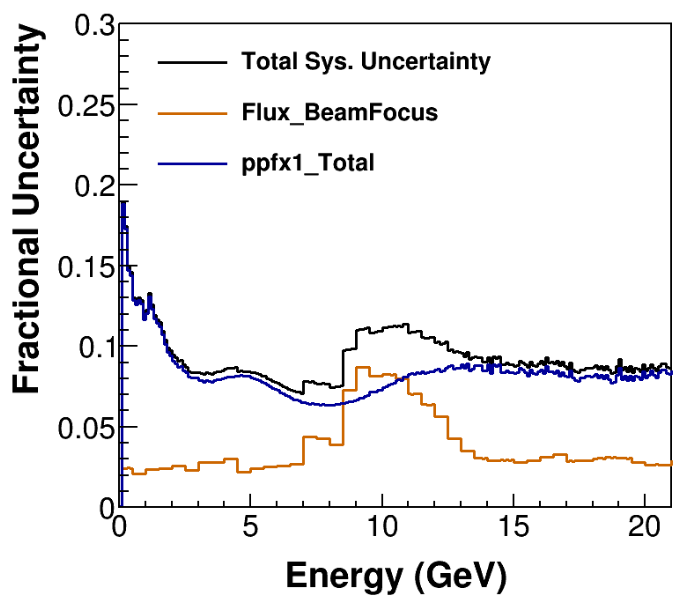
\includegraphics[scale=0.4]{Figures/Chapter6/BeamUncertainties.png}
    \caption{Flux uncertainty breakdown as function of the neutrino energy. The ppfx1\_Total is the total uncertainties produced by the hadron production parameters and the total beam focusing uncertainty. Frigure from \cite{BenThesis}}
    \label{fig:Systematics:FluxUncertainties}
\end{figure} 

The flux uncertainties is one of the biggest components of the total uncertainty in the cross section calculation. For the 1D analysis the variable most affected by this uncertainty is $P^z_\mu$, this uncertainty is between 8\% and 3\% for all the variables. In the 2D analysis the combination of variables more affected is $P^T_\mu$ with $P^z_\mu$. The uncertainty is between 6\% and 3\%. In the \textbf{Appendix} \ref{Ap:Systematics:Flux} the plots with the systematic uncertainties are reported for the 1D and 2D analyses. 

\subsection{Others}
\label{Cap:ErrorAnalysis:SystematicUnc:Others}

This group of uncertainties includes the uncertainties related to the target mass, particle response and the GEANT4 uncertainties. The target mass shifts the density of the material, it changes the deposited energy in the detector. The particle response uncertainties gives information about the calorimetric energy response of the detector, this is specific for each particle. The GEANT4 uncertainties are related to the models that are used to simulate the trajectory of the particles produced in the neutrino interaction and the secondary interactions of the particles in the detector. The

\textcolor{red}{Correr el codigo para obtener el error de GEANT4}



\begin{table}[!htb]
    \centering
    \begin{tabular}{c|p{2in}|c|c|c}
        \hline 
        Parameter & Description.  & Shift (1 $\sigma$) & \multicolumn{2}{c}{Effect} \\
         & & & 1D & 2D \\
        \hline  
        FrPiProd\_N & & $\pm20\%$ & $>2\%$ & $>1.3\%$\\ \hline
        MFP\_N &  & $\pm20\%$ & $>7.2\%$ & $>2.9\%$ \\ \hline
        FrAbs\_N &  & $\pm30\%$ & $>1.7\%$ & $>4\%$ \\ \hline
        FrCEx\_N &  & $\pm50\%$ & $>1.6\%$ & $>1\%$\\ \hline
        FrElas\_N &  & $\pm30\%$ & $>2.5\%$ & $>1.7\%$ \\ \hline
        FrInel\_N &  & $\pm40\%$ & $>2.2\%$ & $>2.1\%$\\ \hline
        
    \end{tabular}
    \caption{The systematic uncertainty description for FSI in nucleons and the effect of it in the cross section results are shown. Based on \cite{GENIEUnc}.}
    \label{tab:ErrorAnalysis:SystematicUnc:Other}
\end{table}


\pagebreak

\section{Cross Section Systematic Uncertainties}
\label{Cap:ErrorAnalysis:CrossSectionUncertainties}

In this section the results for the 1D and the 2D analysis systematic uncertainties summaries is shown. The breakdown plots for each systematic uncertainty can be found in the \textbf{Appendix} \ref{Ap:Systematics}.

\foreach \var in  {enu,mixtpi,mixthetapi_deg,pmu,ptmu,pzmu,thetamu_deg,q2,wexp}{
%\foreach \var in  {enu_true,mixtpi_true,pmu_true,ptmu_true,pzmu_true,thetamu_deg_true,q2_true,wexp_true}{
    \ifthenelse{\equal{\var}{enu}}{
      \renewcommand{\NewVar}{E_\nu}
    }{}
    \ifthenelse{\equal{\var}{mixtpi}}{
      \renewcommand{\NewVar}{T_\pi}
    }{}
    \ifthenelse{\equal{\var}{mixthetapi_deg}}{
      \renewcommand{\NewVar}{\theta_\pi}
    }{}
    \ifthenelse{\equal{\var}{pmu}}{
      \renewcommand{\NewVar}{P_\mu}
    }{}
    \ifthenelse{\equal{\var}{ptmu}}{
      \renewcommand{\NewVar}{P^T_\mu}
    }{}
    \ifthenelse{\equal{\var}{pzmu}}{
      \renewcommand{\NewVar}{P^z_\mu}
    }{}
    \ifthenelse{\equal{\var}{thetamu_deg}}{
      \renewcommand{\NewVar}{\theta_\mu}
    }{}
    \ifthenelse{\equal{\var}{q2}}{
      \renewcommand{\NewVar}{Q^2}
    }{}
    \ifthenelse{\equal{\var}{wexp}}{
      \renewcommand{\NewVar}{W_{exp}}
    }{}
    \begin{figure}
        \centering
        \includegraphics[scale=0.3]{Figures/AppendixB/XsecUnc1D/ErrorSummary_CrossSection_\var_Frac__1Pi_.png}
        \caption{$\NewVar$ 1D Cross Section error summary, including the statistical and systematic uncertainties breakdown per group.}
        \label{fig:Systematics:1DSystematics\var}
    \end{figure}  
}

\foreach \var in  {ptmu_vs_tpi,tpi_vs_ptmu,ptmu_vs_pzmu,pzmu_vs_ptmu,tpi_vs_pmu,pmu_vs_tpi,thetapi_deg_vs_tpi,tpi_vs_thetapi_deg,enu_vs_tpi,tpi_vs_enu}{


    \ifthenelse{\equal{\var}{pzmu_vs_ptmu}}{
      \renewcommand{\NewVar}{P^z_\mu,P^T\mu}
    }{}
    \ifthenelse{\equal{\var}{tpi_vs_thetapi_deg}}{
      \renewcommand{\NewVar}{T_\pi,\theta_\pi}
    }{}
    \ifthenelse{\equal{\var}{tpi_vs_pmu}}{
      \renewcommand{\NewVar}{T_\pi,P_\mu}
    }{}
    \ifthenelse{\equal{\var}{ptmu_vs_tpi}}{
      \renewcommand{\NewVar}{P^T_\mu, T_\pi}
    }{}
    \ifthenelse{\equal{\var}{ptmu_vs_pzmu}}{
      \renewcommand{\NewVar}{P^T\mu, P^z_\mu}
    }{}
    \ifthenelse{\equal{\var}{thetapi_deg_vs_tpi}}{
      \renewcommand{\NewVar}{\theta_\pi, T_\pi}
    }{}
    \ifthenelse{\equal{\var}{pmu_vs_tpi}}{
      \renewcommand{\NewVar}{P_\mu, T\pi}
    }{}
    \ifthenelse{\equal{\var}{tpi_vs_ptmu}}{
      \renewcommand{\NewVar}{T_\pi,P^T_\mu}
    }{}
    \ifthenelse{\equal{\var}{tpi_vs_enu}}{
      \renewcommand{\NewVar}{T_\pi,E_\nu}
    }{}
    \ifthenelse{\equal{\var}{enu_vs_tpi}}{
      \renewcommand{\NewVar}{E_\nu, T_\pi}
    }{}
    \begin{figure}
        \centering
        \includegraphics[scale=0.3]{Figures/AppendixB/XsecUnc2D/2D_ErrorSummary_CrossSection_\var_.png}
        \caption{$\NewVar$ 2D Cross Section error summary, including the statistical and systematic uncertainties breakdown per group.}
        \label{fig:Systematics:2DSystematics\var}
    \end{figure}  
}
